\chapter{參數評估模擬案例與成果探討}
\fontsize{12pt}{18pt}\selectfont

% ------------------------- 5.0 ------------------------- %
% 概述;本章安排
上一章完成了模擬案例的前置作業,本章節將根據問題複雜度分類,透過多運動軌跡預測最佳化對每個案例進行參數估計,
藉由上肢模型來實現所提出之研究方法,接續將針對評估結果進行討論,並從預測結果與參數結果的兩個面向進行切入,
最後對單軌跡案例的模擬結果來探討,以參數不可識別性為主軸來描述其對參數評估的影響。

% ------------------------- 5.1 ------------------------- %
\section{參數評估模擬案例}
% 針對二頭肌探討;研究案例分類;前三個案例用"多軌跡";額外的案例用"單軌跡"
本節將綜合成果來展示數個模擬案例,透過最佳化方法來評估肱二頭肌群的肌肉參數,
下方圖 \ref{ch5_flowchart_StudyCase} 為本研究案例分類,主要以評估的參數數量來區分,
其皆是透過「多」運動軌跡預測最佳化來進行評估,另外將會補充一個以「單」運動軌跡預測最佳化評估的單軌跡案例,
屆時會透過此案例來體現多預測任務的重要性。

% 案例任務使用
在單肌肉單參數案例、單肌肉多參數案例和多肌肉多參數案例皆是使用多預測任務來執行,統稱為多軌跡案例,
代表在最佳化搜尋時必須同時滿足上一章節所選定的兩項任務 (Task 7 與 Task 8), 
而在單軌跡案例中則是使用單預測任務,所挑選使用的任務為 Task 7。 

\clearpage

\begin{figure}[!ht]
	\centering
	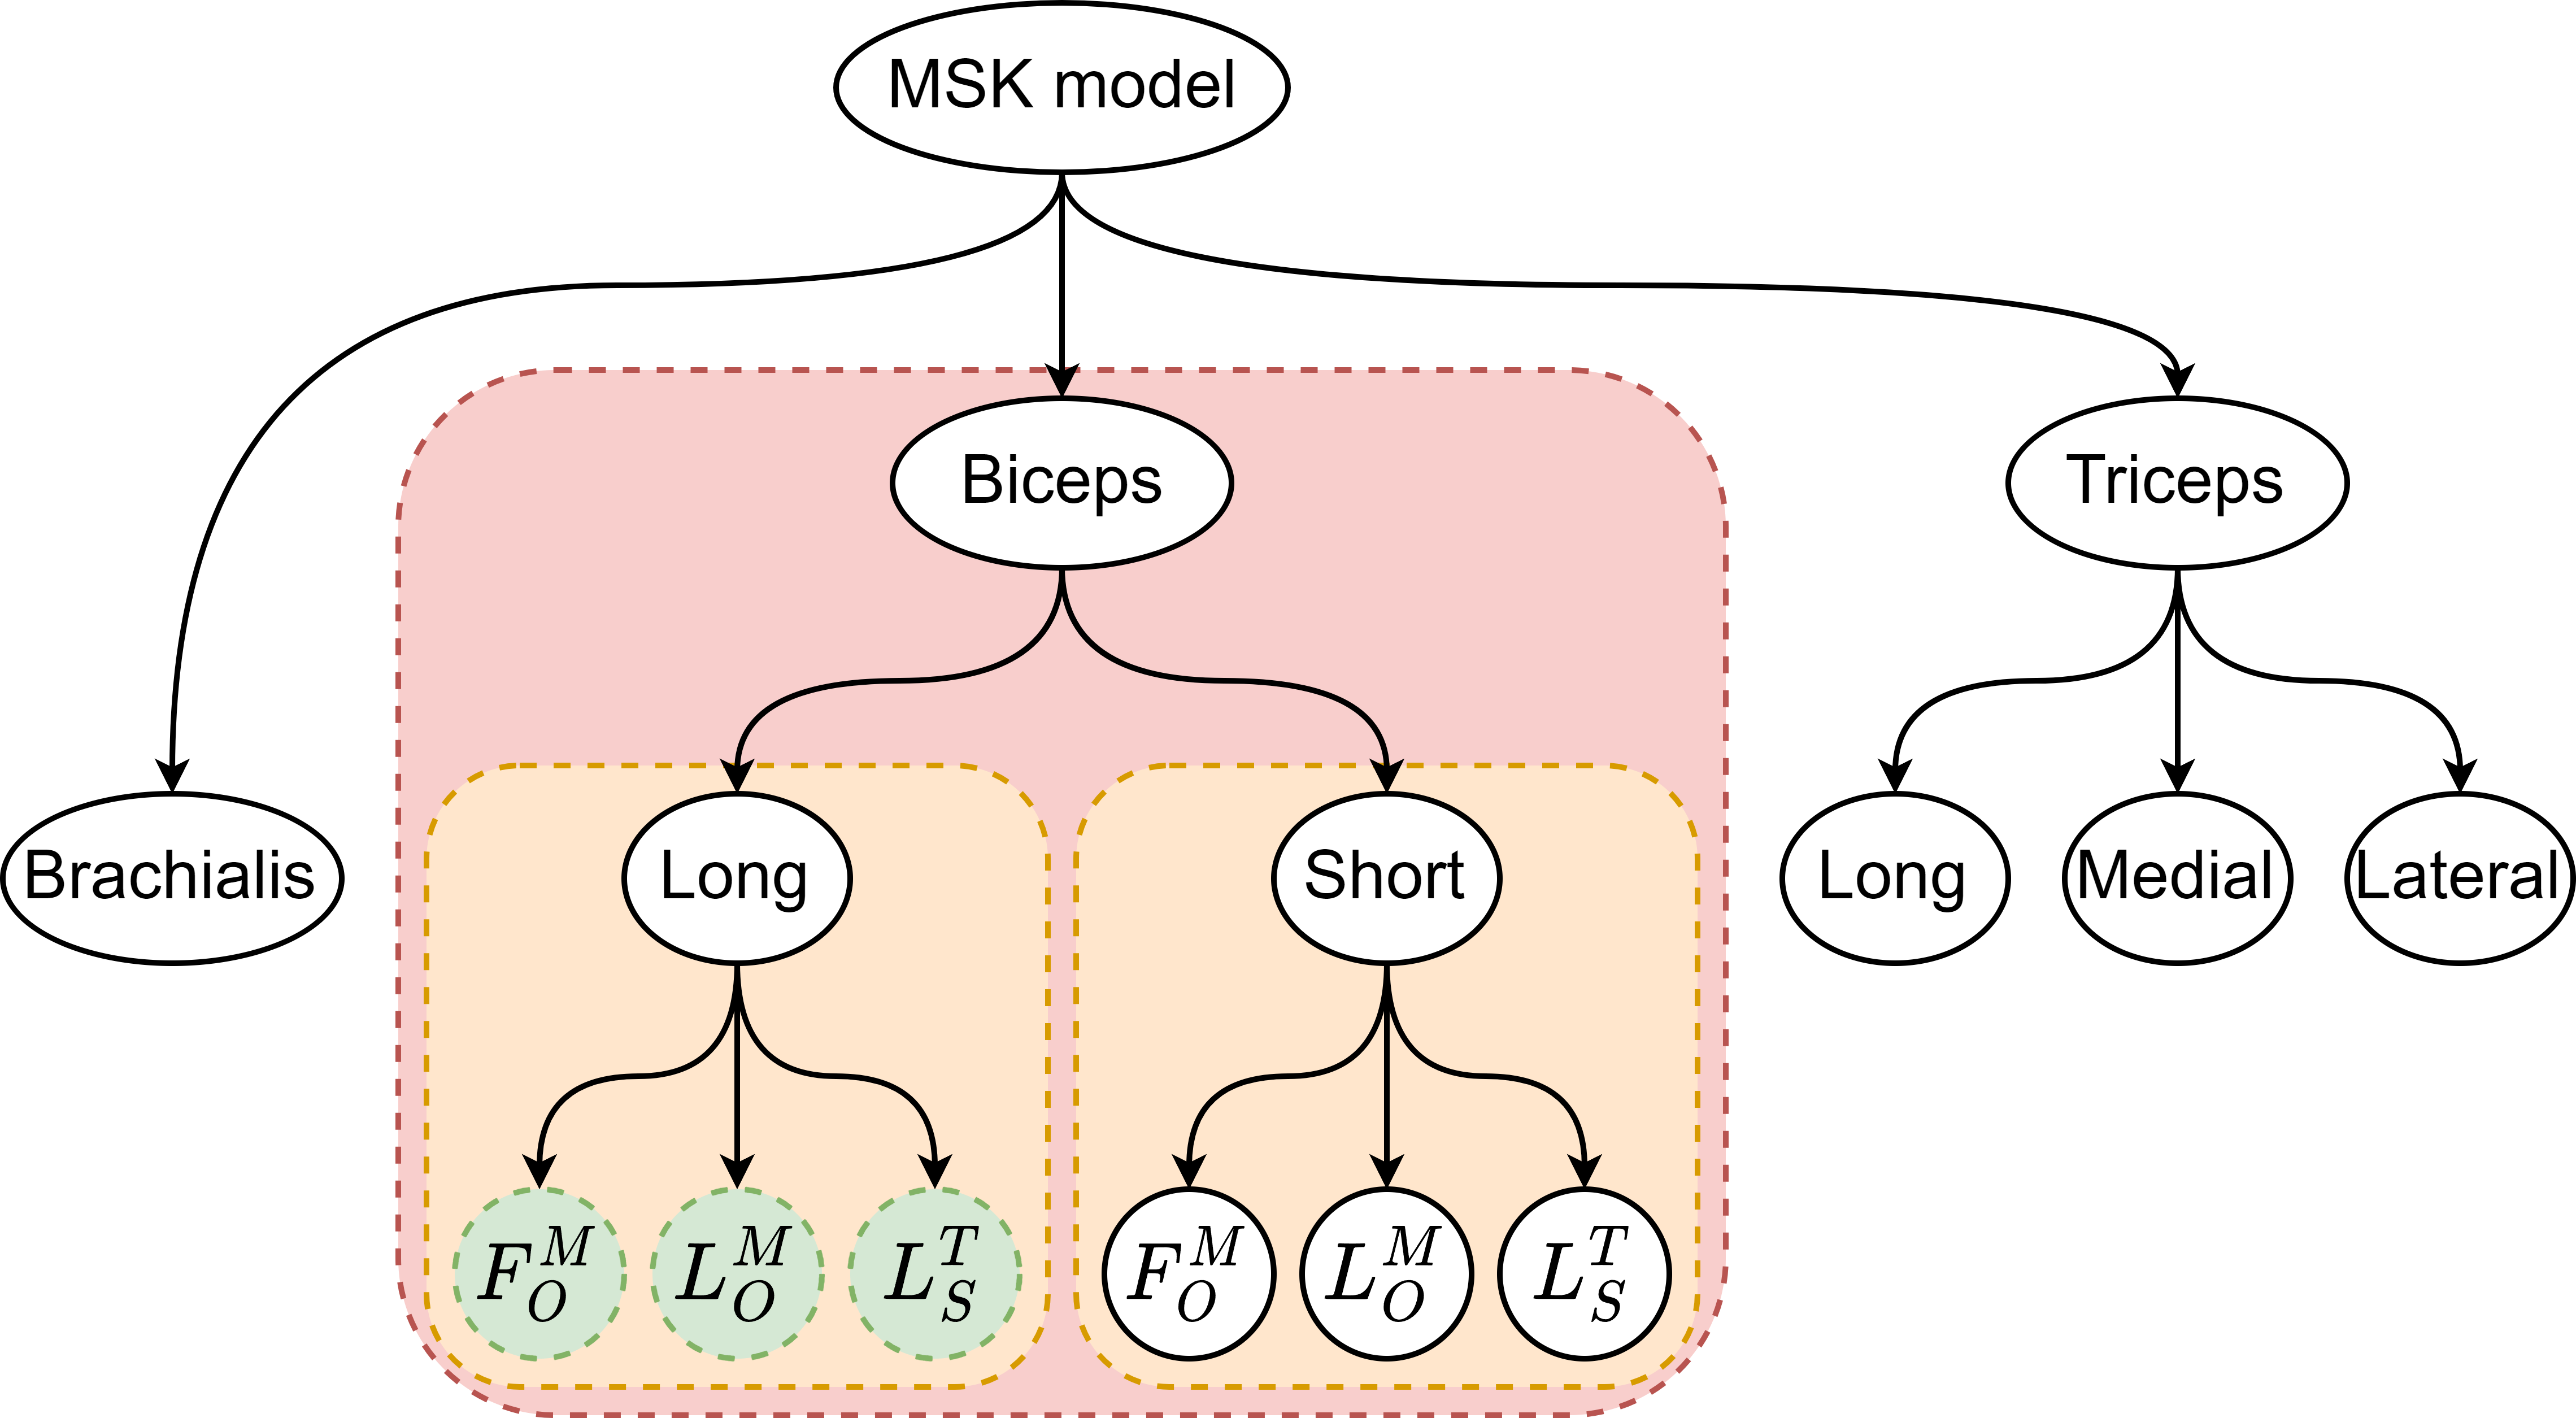
\includegraphics[width=13cm]{figure/ch5_flowchart_StudyCase.png}
    \caption[研究案例分類]{研究案例分類,其中
                          綠色代表評估單一肌肉之單一參數,含有 1 個設計變數,即單肌肉單參數案例;
                          橘色代表評估單一肌肉之多參數,含有 3 個設計變數,即單肌肉多參數案例;
                          紅色代表評估多肌肉之多參數,含有 6 個設計變數,即多肌肉多參數案例。}
    \label{ch5_flowchart_StudyCase}
\end{figure}

\subsection{單肌肉單參數案例評估}
% 肱二頭肌長頭;一個參數
單肌肉單參數案例將對單一肌肉之單一參數進行評估,意味著最佳化問題中含有 1 個設計變數,而非設計變數的肌肉參數則維持為預設值,
下方以「肱二頭肌長頭的三個肌肉參數」作為評估範例,個別執行參數最佳化與模型驗證,總共含有三個例子展示。

\subsubsection{肱二頭肌長頭之最大等長力量}
% 評估結果 (Opt/Vali 的 NRMSE);表:參數結果
最佳化演算法得到的最小誤差為 $E^\mathrm{mean}_\mathrm{NRMSE} = \frac{4.40 \times 10^{-5} + 4.20 \times 10^{-5}}{2} = 4.30 \times 10^{-5}$,
所得到對應的最佳參數如表 \ref{ch5_table_Case1_FMO} 所示,
其中尋找初始值與最佳解的迭代過程各花了 23 秒與 76 秒的執行時間,
而最佳模型執行驗證任務的結果為 $E_\mathrm{NRMSE} = 2 \times 10^{-4}$。

\begin{table}[!ht]
    \caption[單肌肉單參數案例:肱二頭肌長頭之最大等長力量的最佳參數]{單肌肉單參數案例於肱二頭肌長頭之最大等長力量的最佳參數}
	\label{ch5_table_Case1_FMO}
	\centering
    \setlength{\tabcolsep}{16pt}{
    \renewcommand\arraystretch{1.5}{ % 縱向
    \begin{tabular}{l|c}
        Muscle name  & $F^\mathrm{M}_\mathrm{O}$ (N) \\ \hline\hline
        BIClong      & 624.302
    \end{tabular}}}
\end{table}

\clearpage

\subsubsection{肱二頭肌長頭之最佳肌纖維長度}
% 評估結果 (Opt/Vali 的 NRMSE);表:參數結果
最佳化演算法得到的最小誤差為 $E^\mathrm{mean}_\mathrm{NRMSE} = \frac{5.10 \times 10^{-5} + 5.40 \times 10^{-5}}{2} = 5.25 \times 10^{-5}$,
所得到對應的最佳參數如表 \ref{ch5_table_Case1_LMO} 所示,
其中尋找初始值與最佳解的迭代過程各花了 6 秒與 33 秒的執行時間,
而最佳模型執行驗證任務的結果為 $E_\mathrm{NRMSE} = 6.00 \times 10^{-4}$。

\begin{table}[!ht]
    \caption[單肌肉單參數案例:肱二頭肌長頭之最佳肌纖維長度的最佳參數]{單肌肉單參數案例於肱二頭肌長頭之最佳肌纖維長度的最佳參數}
	\label{ch5_table_Case1_LMO}
	\centering
    \setlength{\tabcolsep}{16pt}{
    \renewcommand\arraystretch{1.5}{ % 縱向
    \begin{tabular}{l|c}
        Muscle name  & $L^\mathrm{M}_\mathrm{O}$ (m) \\ \hline\hline
        BIClong      & 0.11570
    \end{tabular}}}
\end{table}

\subsubsection{肱二頭肌長頭之肌腱鬆弛長度}
% 評估結果 (Opt/Vali 的 NRMSE);表:參數結果
最佳化演算法得到的最小誤差為 $E^\mathrm{mean}_\mathrm{NRMSE} = \frac{4.50 \times 10^{-5} + 4.50 \times 10^{-5}}{2} = 4.50 \times 10^{-5}$,
所得到對應的最佳參數如表 \ref{ch5_table_Case1_LTS} 所示,
其中尋找初始值與最佳解的迭代過程各花了 6 秒與 42 秒的執行時間,
而最佳模型執行驗證任務的結果為 $E_\mathrm{NRMSE} = 3 \times 10^{-4}$。

\begin{table}[!ht]
    \caption[單肌肉單參數案例:肱二頭肌長頭之肌腱鬆弛長度的最佳參數]{單肌肉單參數案例於肱二頭肌長頭之肌腱鬆弛長度的最佳參數}
	\label{ch5_table_Case1_LTS}
	\centering
    \setlength{\tabcolsep}{16pt}{
    \renewcommand\arraystretch{1.5}{ % 縱向
    \begin{tabular}{l|c}
        Muscle name  & $L^\mathrm{T}_\mathrm{S}$ (m) \\ \hline\hline
        BIClong      & 0.27230
    \end{tabular}}}
\end{table}

\subsection{單肌肉多參數案例評估}
% 肱二頭肌長頭/短頭;三個參數
單肌肉多參數案例將對單一肌肉之多參數進行評估,意味著最佳化問題中含有 3 個設計變數,而非設計變數的肌肉參數則維持為預設值,
下方以「肱二頭肌長頭」與「肱二頭肌短頭」作為評估範例,個別執行參數最佳化與模型驗證,總共含有兩個例子展示。

\subsubsection{肱二頭肌長頭}
% 評估結果 (Opt/Vali 的 NRMSE);表:參數結果
最佳化演算法得到的最小誤差為 $E^\mathrm{mean}_\mathrm{NRMSE} = \frac{4.20 \times 10^{-5} + 6.00 \times 10^{-5}}{2} = 5.10 \times 10^{-5}$,
所得到對應的最佳參數如表 \ref{ch5_table_Case2_Long} 所示,
其中尋找初始值與最佳解的迭代過程各花了 217 秒與 303 秒的執行時間,
而最佳模型執行驗證任務的結果為 $E_\mathrm{NRMSE} = 4.00 \times 10^{-4}$。

\begin{table}[!ht]
    \caption[單肌肉多參數案例:肱二頭肌長頭的最佳參數]{單肌肉多參數案例於肱二頭肌長頭的最佳參數}
	\label{ch5_table_Case2_Long}
	\centering
    \setlength{\tabcolsep}{16pt}{
    \renewcommand\arraystretch{1.5}{ % 縱向
    \begin{tabular}{l|ccc}
        Muscle name  & $F^\mathrm{M}_\mathrm{O}$ (N) & $L^\mathrm{M}_\mathrm{O}$ (m) & $L^\mathrm{T}_\mathrm{S}$ (m) \\ \hline\hline
        BIClong      & 624.326 & 0.11568 & 0.27230
    \end{tabular}}}
\end{table}

\subsubsection{肱二頭肌短頭}
% 評估結果 (Opt/Vali 的 NRMSE);表:參數結果
最佳化演算法得到的最小誤差為 $E^\mathrm{mean}_\mathrm{NRMSE} = \frac{7.40 \times 10^{-5} + 5.20 \times 10^{-5}}{2} = 6.3 \times 10^{-5}$,
所得到對應的最佳參數如表 \ref{ch5_table_Case2_Short} 所示,
其中尋找初始值與最佳解的迭代過程各花了 451 秒與 530 秒的執行時間,
而最佳模型執行驗證任務的結果為 $E_\mathrm{NRMSE} = 2.10 \times 10^{-3}$。

\begin{table}[!ht]
    \caption[單肌肉多參數案例:肱二頭肌短頭的最佳參數]{單肌肉多參數案例於肱二頭肌短頭的最佳參數}
	\label{ch5_table_Case2_Short}
	\centering
    \setlength{\tabcolsep}{16pt}{
    \renewcommand\arraystretch{1.5}{ % 縱向
    \begin{tabular}{l|ccc}
        Muscle name  & $F^\mathrm{M}_\mathrm{O}$ (N) & $L^\mathrm{M}_\mathrm{O}$ (m) & $L^\mathrm{T}_\mathrm{S}$ (m) \\ \hline\hline
        BICshort     & 435.586 & 0.13208 & 0.19230
    \end{tabular}}}
\end{table}

\subsection{多肌肉多參數案例評估}
% 肱二頭肌群;六個參數
多肌肉多參數案例將對多肌肉之多參數進行評估,意味著最佳化問題中含有 $3 \times N_\mathrm{m}$ 個設計變數,
而非設計變數的肌肉參數則維持為預設值,下方以「肱二頭肌群」作為評估範例 (6 個設計變數),執行參數最佳化與模型驗證。

\subsubsection{肱二頭肌群}
% 評估結果 (Opt/Vali 的 NRMSE);表:參數結果
最佳化演算法得到的最小誤差為 $E^\mathrm{mean}_\mathrm{NRMSE} = \frac{1.04 \times 10^{-4} + 1.11 \times 10^{-4}}{2} = 1.08 \times 10^{-4}$,
所得到對應的最佳參數如表 \ref{ch5_table_Case3_BICs} 所示,
其中尋找初始值與最佳解的迭代過程各花了 1223 秒與 3420 秒的執行時間,
而最佳模型執行驗證任務的結果為 $E_\mathrm{NRMSE} = 5.60 \times 10^{-3}$。

\begin{table}[!ht]
    \caption[多肌肉多參數案例:肱二頭肌群的最佳參數]{多肌肉多參數案例於肱二頭肌群的最佳參數}
	\label{ch5_table_Case3_BICs}
	\centering
    \setlength{\tabcolsep}{16pt}{
    \renewcommand\arraystretch{1.5}{ % 縱向
    \begin{tabular}{l|ccc}
        Muscle name  & $F^\mathrm{M}_\mathrm{O}$ (N) & $L^\mathrm{M}_\mathrm{O}$ (m) & $L^\mathrm{T}_\mathrm{S}$ (m) \\ \hline\hline
        BIClong      & 624.601 & 0.11560 & 0.27236 \\ \hline
        BICshort     & 435.264 & 0.13206 & 0.19231
    \end{tabular}}}
\end{table}

\clearpage

\subsection{單軌跡案例評估}
% 肱二頭肌群;六個參數;僅執行一個預測任務 (Task 7)
單軌跡案例為多肌肉多參數案例之變形,僅差異在單軌跡案例為執行單個預測任務 (Task 7),是以單運動軌跡預測最佳化來評估肌肉參數,
下方同樣以「肱二頭肌群」作為評估範例 (6 個設計變數),執行後續的參數最佳化與模型驗證。

\subsubsection{肱二頭肌群}
% 評估結果 (Opt/Vali 的 NRMSE);表:參數結果
最佳化演算法得到的最小誤差為 $E^\mathrm{mean}_\mathrm{NRMSE} = 5.14 \times 10^{-3}$,
所得到對應的最佳參數如表 \ref{ch5_table_CaseE_BICs} 所示,
其中尋找初始值與最佳解的迭代過程各花了 1247 秒與 1215 秒的執行時間,
而最佳模型執行驗證任務的結果為 $E_\mathrm{NRMSE} = 6.86 \times 10^{-1}$。

\begin{table}[!ht]
    \caption[單軌跡案例:肱二頭肌群的最佳參數]{單軌跡案例於肱二頭肌群的最佳參數}
	\label{ch5_table_CaseE_BICs}
	\centering
    \setlength{\tabcolsep}{16pt}{
    \renewcommand\arraystretch{1.5}{ % 縱向
    \begin{tabular}{l|ccc}
        Muscle name  & $F^\mathrm{M}_\mathrm{O}$ (N) & $L^\mathrm{M}_\mathrm{O}$ (m) & $L^\mathrm{T}_\mathrm{S}$ (m) \\ \hline\hline
        BIClong      & 574.490 & 0.13464 & 0.23260 \\ \hline
        BICshort     & 356.981 & 0.10780 & 0.19486
    \end{tabular}}}
\end{table}

% ------------------------- 5.2 ------------------------- %
\section{參數評估結果}
% 參數誤差計算方法
下方表格 \ref{ch5_table_Case123_Results} 為多軌跡案例的參數評估結果整理,
除了上一節就有提供的最佳化最小誤差 (平均誤差) 與模型驗證誤差外,還新增了一項「參數誤差」,乃是因為本研究呈現的是模擬案例,
故有參數結果的標準答案,即原先模型的預設參數值 (表 \ref{ch4_table_ModelDefaultParam})。
參數誤差的計算方法是先取得每項參數與標準答案的誤差百分比絕對值,再將全部結果取平均,如單肌肉單參數案例只有一項最佳參數,
則參數誤差即為該項參數與標準答案的誤差百分比,而如多肌肉多參數案例其最佳參數含有六項,則是將各個參數的誤差取平均。

% 表格:多軌跡案例結果
\begin{table}[!ht]
    \caption[多軌跡案例之肌肉參數評估成果整理]{多軌跡案例之肌肉參數評估成果整理}
	\label{ch5_table_Case123_Results}
    \centering
    \begin{adjustbox}{angle=90}
    \setlength{\tabcolsep}{10pt}{
    \renewcommand\arraystretch{1.5}{ % 縱向
    \begin{tabular}{ll|ccc}
                                        &               & \multicolumn{1}{c}{\begin{tabular}[c]{@{}c@{}} 最佳化最小誤差 \\ $E^\mathrm{mean}_\mathrm{NRMSE}$ \end{tabular}} & \multicolumn{1}{c}{\begin{tabular}[c]{@{}c@{}} 模型驗證誤差 \\ $E_\mathrm{NRMSE}$ \end{tabular}} & \multicolumn{1}{c}{參數誤差} \\ \hline\hline
        \multirow{3}{*}{單肌肉單參數案例} & 最大等長力量   & $4.30 \times 10^{-5}$ & $2.00 \times 10^{-4}$ & $3.20 \times 10^{-6}$  \\
                                         & 最佳肌纖維長度 & $5.25 \times 10^{-5}$ & $6.00 \times 10^{-4}$ & $ < 4.24 \times 10^{-5}$  \\
                                         & 肌腱鬆弛長度   & $4.50 \times 10^{-5}$ & $3.00 \times 10^{-4}$ & $ < 1.80 \times 10^{-5}$  \\ \hline
        \multirow{2}{*}{單肌肉多參數案例} & 肱二頭肌長頭   & $5.10 \times 10^{-5}$ & $4.00 \times 10^{-4}$ & $7.15 \times 10^{-5}$  \\
                                         & 肱二頭肌短頭   & $6.30 \times 10^{-5}$ & $2.10 \times 10^{-3}$ & $7.04 \times 10^{-5}$  \\ \hline
        多肌肉多參數案例                  & 肱二頭肌群     & $1.08 \times 10^{-4}$ & $5.60 \times 10^{-3}$ & $4.34 \times 10^{-4}$
    \end{tabular}}}
    \end{adjustbox}
\end{table}

% 多軌跡案例
從多軌跡案例的結果顯示,最佳化演算法皆中斷於極小的平均誤差值,而用來確認最佳模型的間接驗證方法,
也都呈現著良好的預測成效,至此可大致確定每個案例的最佳參數組合與標準答案有高度相似,
最終從參數誤差項也直接驗證結果,故所提出的研究方法能有效地估計肌肉參數。

\clearpage

% ------------------------- 5.3 ------------------------- %
\section{肌肉參數不可識別性探討}
% 單軌跡案例
本節將以單軌跡案例結果來探討關於肌肉參數不可識別性問題,表 \ref{ch5_table_CaseE_Results} 為單軌跡案例的評估成果整理,
數據顯示最佳化演算法雖未如先前案例尋找到極小值,不過該誤差仍非常小,
下方圖 \ref{ch5_fig_CaseE_BICs_7} 與 \ref{ch5_fig_CaseE_BICs_40} 則為單軌跡案例所得到之最佳模型所執行的軌跡預測圖,
於常理來說,最佳參數應於驗證模型時仍具有低預測誤差的表現,但結果並非如此,
而參數誤差項也證實了該組最佳參數距離標準答案甚遠,此評估結果意味著這組最佳參數在最佳化任務中能達成精準預測,
但於其他任務中卻無法有同樣的預測能力,可得知若是預測任務不夠明確與多樣,將會造成模型具有多組解的情況發生,
如文獻探討所提及之肌肉代償、參數抗衡等問題。

% 表格:單軌跡案例結果
\begin{table}[!ht]
    \caption[單軌跡案例之肌肉參數評估成果整理]{單軌跡案例之肌肉參數評估成果整理}
	\label{ch5_table_CaseE_Results}
	\centering
    \setlength{\tabcolsep}{10pt}{
    \renewcommand\arraystretch{1.5}{ % 縱向
    \begin{tabular}{ll|ccc}
                 &           & \multicolumn{1}{c}{\begin{tabular}[c]{@{}c@{}} 最佳化最小誤差 \\  $E^\mathrm{mean}_\mathrm{NRMSE}$ \end{tabular}} & \multicolumn{1}{c}{\begin{tabular}[c]{@{}c@{}} 模型驗證誤差 \\ $E_\mathrm{NRMSE}$ \end{tabular}} & \multicolumn{1}{c}{參數誤差} \\ \hline\hline
        單軌跡案例  & 肱二頭肌群 & $5.14 \times 10^{-3}$ & $6.86 \times 10^{-1}$ & $1.28 \times 10^{-1}$
        \end{tabular}}}
\end{table}

\begin{figure}[!ht]
	\centering
	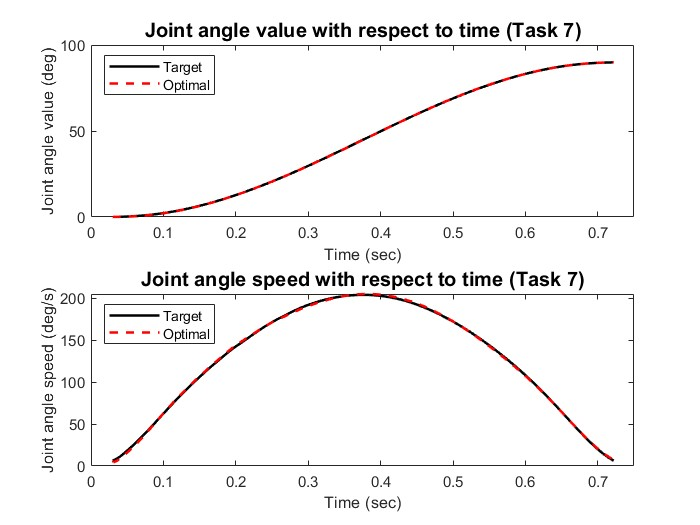
\includegraphics[width=13cm]{figure/ch5_fig_CaseE_BICs_Opt_7.JPG}
    \caption[單軌跡案例於最佳化任務之運動軌跡預測]{單軌跡案例於最佳化任務 (Task 7) 之運動學軌跡預測,
                                              包含關節轉動角度與關節轉動速度對時間之關係。}
    \label{ch5_fig_CaseE_BICs_7}
\end{figure}

\clearpage

\begin{figure}[!ht]
	\centering
    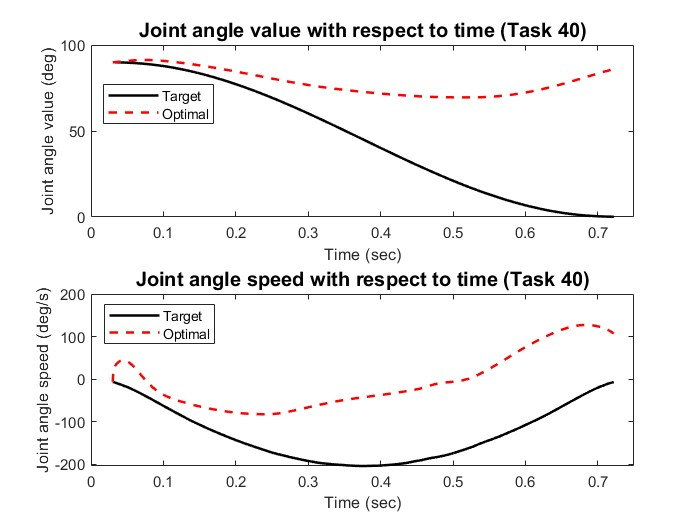
\includegraphics[width=13cm]{figure/ch5_fig_CaseE_BICs_Vali_40.JPG}
    \caption[單軌跡案例於模型驗證任務之運動軌跡預測]{單軌跡案例於模型驗證任務 (Task 40) 之運動學軌跡預測,
                                                包含關節轉動角度與關節轉動速度對時間之關係。}
    \label{ch5_fig_CaseE_BICs_40}
\end{figure}

\begin{figure}[!ht]
	\centering
	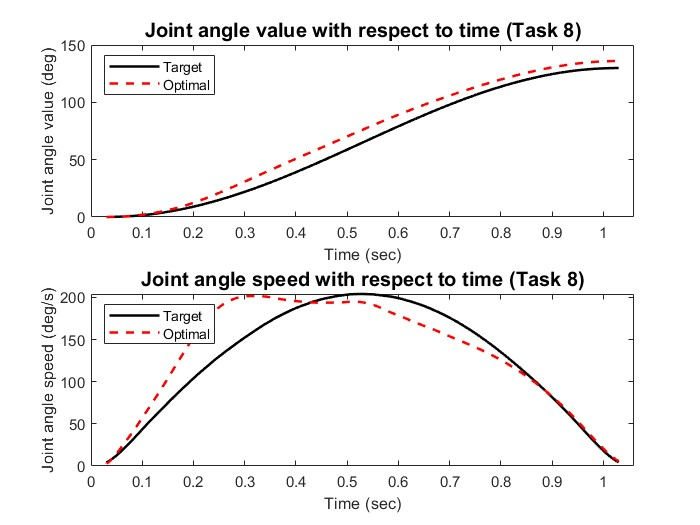
\includegraphics[width=13cm]{figure/ch5_fig_CaseE_BICs_Opt_8.JPG}
    \caption[單軌跡案例於 Task 8 之運動軌跡預測]{透過單軌跡案例得到的最佳模型來額外執行 Task 8 之運動學軌跡預測,
                                             包含關節轉動角度與關節轉動速度對時間之關係。}
    \label{ch5_fig_CaseE_BICs_8}
\end{figure}

\clearpage

% 討論
在上方單軌跡案例中,結果可能會找到軌跡預測誤差極小的解,但該組解卻離標準答案甚遠,
不能把這種情況歸咎於最佳化演算法的問題,演算法確實找到一組極小的答案並停止迭代,但不幸的是該組解為較遠的局部最小值,
不管是在肌肉與肌肉間的代償關係,還是在希爾式肌肉模型中的參數抗衡,皆會影響肌肉參數評估的準確性,
因此加入其餘軌跡的預測是必要的,使尋找到的最佳模型能同時完成多個預測任務,也使最佳化問題中的目標函數更加明確。
如上方圖 \ref{ch5_fig_CaseE_BICs_8} 為透過單軌跡案例得到的最佳模型,來額外執行多肌肉多參數案例的第二個最佳化任務 (Task 8),
從單軌跡案例得到的最佳模型在 Task 8 中仍然表現不佳,若如多肌肉多參數案例同時評估 Task 7 與 Task 8 兩個任務,即可以解決上述問題。 

% 最小誤差判定
另外在最佳化演算法上,很難僅透過最小誤差來判定尋找到的參數結果是否正確,最小誤差與參數誤差由於參數不可識別性的影響,
兩者並非呈現正相關的關係,無法訂定一個最小誤差的閾值來作為最佳化演算法的停止條件。舉例來說,
將二頭肌群在表 \ref{ch4_table_ModelDefaultParam} 的 6 個預設參數值進行偏移,分別全部偏移 $+ 1\%$ 與 $- 1\%$,
也就是參數誤差皆為 $1 \times 10^{-2}$,在這兩種情形執行 Task 7 下,預測誤差分別為 $2.90 \times 10^{-2}$ 和 $1.98 \times 10^{-2}$,
與先前介紹的單軌跡案例相比 (參數誤差 $1.28 \times 10^{-1}$;最小誤差/預測誤差 $5.14 \times 10^{-3}$),
即可發現單軌跡案例縱使有較大的參數誤差 (距離標準答案較遠),在 Task 7 卻有著更小的預測誤差結果。
結論為在最佳化過程中,並不能在演算法終止條件上設定目標函數的閾值,而得到的最佳解必須透過模型驗證過程來確認是否正確。

% ------------------------- 5.4 ------------------------- %
\section{小結}
% 總結
本章節透過常見的上肢骨骼模型作為模擬範例,來展示最佳化與間接驗證方法,並根據結果來針對每個案例進行深入探討。
本論文由於皆為模擬研究的緣故,最佳參數可與真實答案 (參數預設值) 進行比較,綜合多軌跡案例的模型驗證與參數誤差結果,
提出的方法能有效地找到肌肉骨骼模型中之指定的肌肉肌腱參數,證實該方法能應用於個人化模型的建立,另外在單軌跡案例中,
最佳化迭代中止且得到的預測誤差很小,但在模型驗證階段卻有巨大的預測誤差,透過該現象來探討關於參數不可識別性的問題,
並說明了多預測任務的必要性。下一章節將統整整篇論文的結論與貢獻,並提出相關之未來工作。

\clearpage